\section{Cálculo por Elementos Finitos de la fuerza de atracción}
\label{sec:simulaciones}

En esta sección, se describe el proceso de creación del modelo de la lanzadera electromagnética realizado utilizando ANSYS Maxwell\textsuperscript{\textregistered}. Este software de métodos finitos está especializado en el análisis de sistemas electromagnéticos. El objetivo de estas simulaciones es obtener una comprensión detallada del comportamiento del campo magnético generado por la bobina y su interacción con el proyectil ferromagnético en la lanzadera electromagnética. Se ha dividido el proceso en tres subapartados: creación de la geometría, simulaciones instantáneas y simulaciones transitorias. En la primera, se mostrará el proceso de creación de la geometría paramétrica en 2D y 3D, en la segunda y tercera se explicarán las condiciones de contorno y resultados de las simulaciones instantáneas y transitorias, respectivamente. En el Anexo III se detalla el procedimiento de creación de la geometría y realización de simulaciones.

\subsection{Geometría}
El primer paso para realizar las simulaciones fue la creación de la geometría del sistema en ANSYS Maxwell\textsuperscript{\textregistered}. Para ello, se definieron las dimensiones y características de la bobina y el proyectil de manera paramétrica. Esto quiere decir que las dimensiones de los polígonos que conforman el modelo no son fijas, si no que están asociadas a variables por lo que simular diferentes configuraciones se convierte en algo más sencillo. La geometría fue primeramente diseñada en 3D, pero también se obtuvo la sección central del archivo tridimensional para poder simular en 2D, lo que permite realizar las simulaciones con un menor tiempo de computación. Una vez creada la geometría, se definieron los diferentes materiales y sus propiedades electromagnéticas. El material utilizado para los conductores del solenoide es cobre recocido, PVC para el soporte de la bobina y acero F114 para el vástago. Con esto, se modela la geometría a continuación mostrada:

\begin{itemize}
    \item \textbf{Geometría en 3D}:
    \begin{figure}[H]
        \centering
        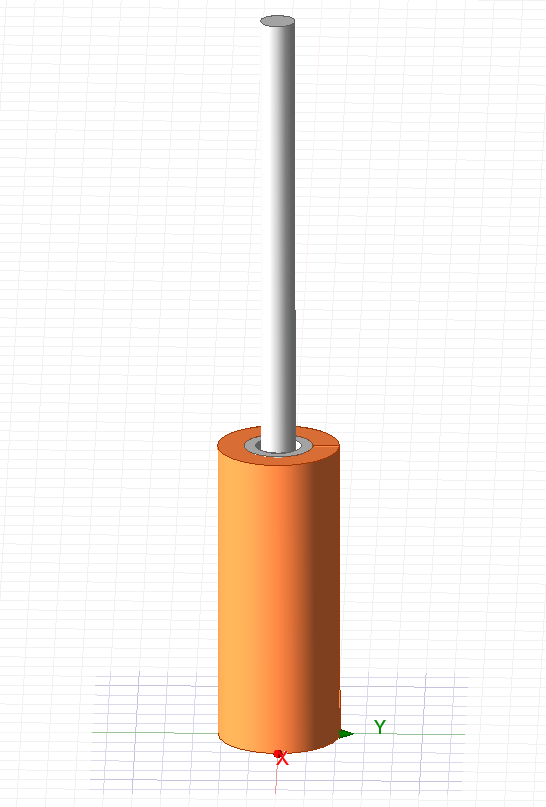
\includegraphics[width=6.7cm]{FigurasMemoria/geom3d.png}
        \caption{Geometría de la barra y bobina en 3D.}
        \label{fig:geom3d} %Para referenciar -> \ref{fig:figNum}
    \end{figure}
    \item \textbf{Mallado en 3D}:
    \begin{figure}[H]
        \centering
        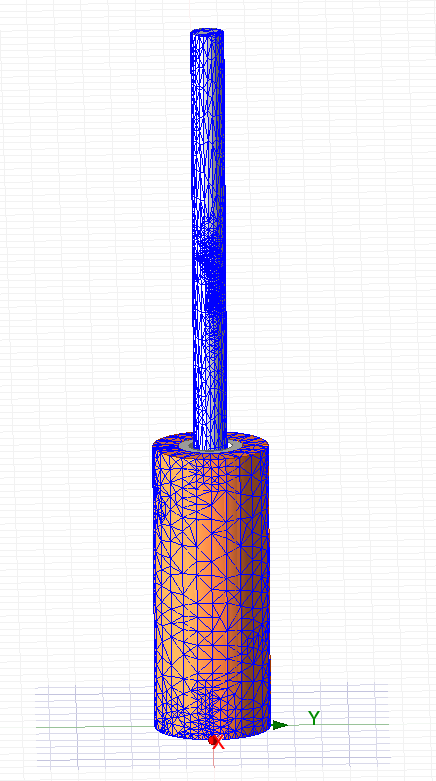
\includegraphics[width=7cm]{FigurasMemoria/mesh3d.png}
        \caption{Mallado de la barra y bobina en 3D.}
        \label{fig:mesh3d} %Para referenciar -> \ref{fig:figNum}
    \end{figure}
    \begin{figure}[H]
        \centering
        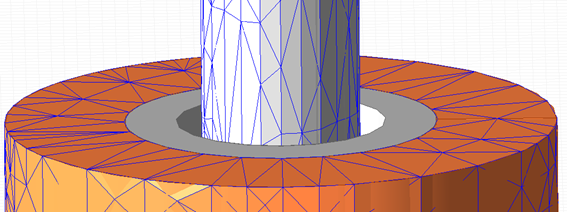
\includegraphics[width=9cm]{FigurasMemoria/meshDetail3d.png}
        \caption{Detalle del mallado de la barra y bobina en 3D.}
        \label{fig:meshDetail3d} %Para referenciar -> \ref{fig:figNum}
    \end{figure}

    \vspace{5cm}
    
    \item \textbf{Geometría en 2D}:
    \begin{figure}[H]
        \centering
        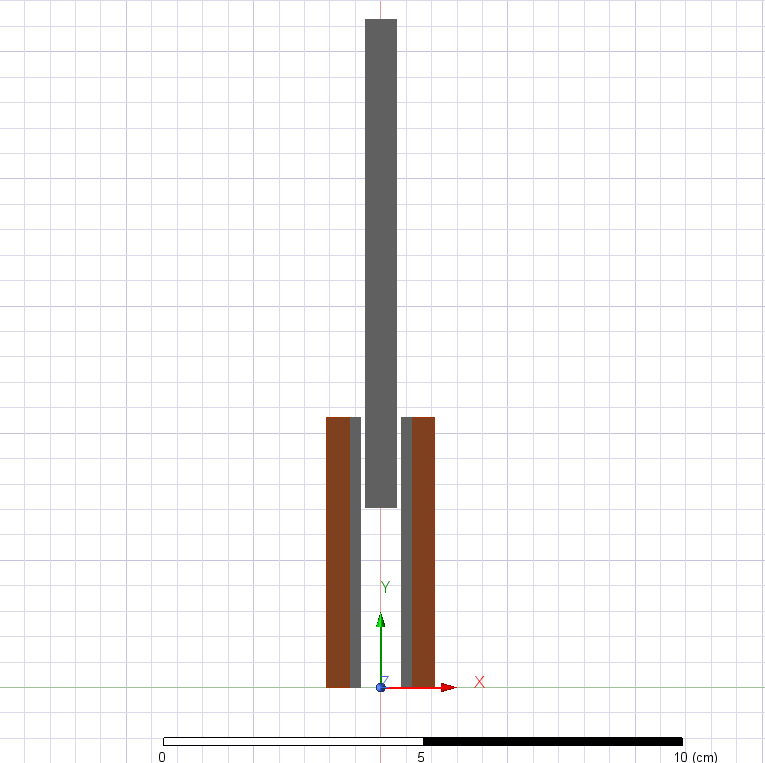
\includegraphics[width=9cm]{FigurasMemoria/BarGeom.png}
        \caption{Geometría de la barra y bobina en 2D.}
        \label{fig:BarGeom} %Para referenciar -> \ref{fig:figNum}
    \end{figure}
    \item \textbf{Mallado en 2D}:
    \begin{figure}[H]
        \centering
        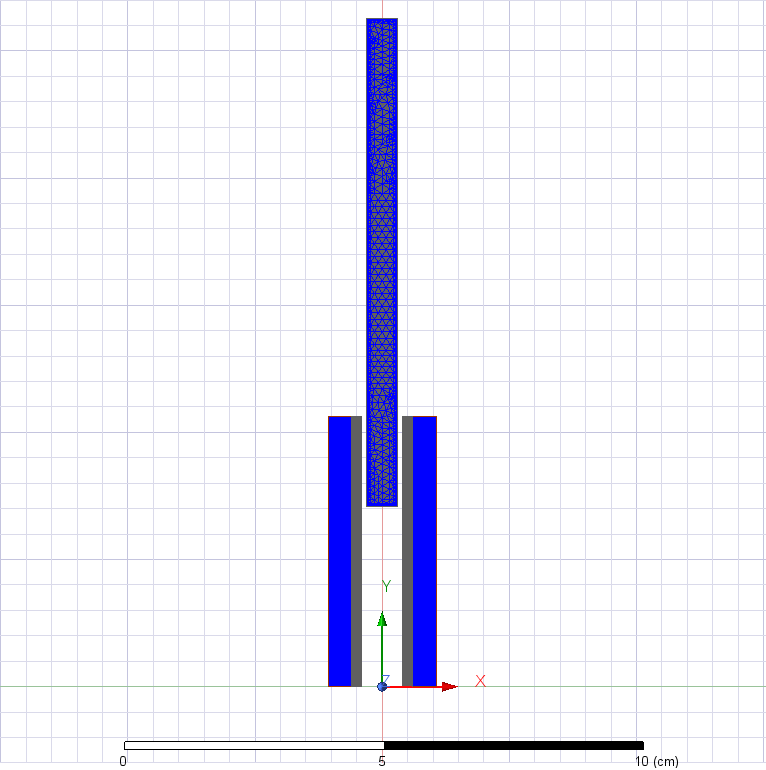
\includegraphics[width=9cm]{FigurasMemoria/BarGeomMesh.png}
        \caption{Mallado de la barra y bobina en 2D.}
        \label{fig:BarGeomMesh} %Para referenciar -> \ref{fig:figNum}
    \end{figure}
    \begin{figure}[H]
        \centering
        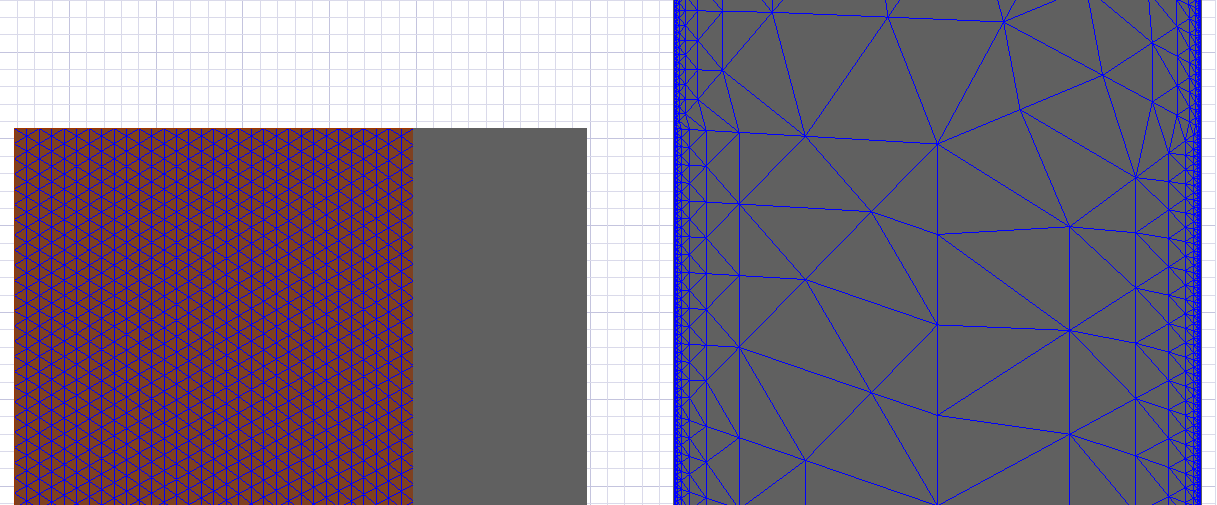
\includegraphics[width=9cm]{FigurasMemoria/BarMeshDetail.png}
        \caption{Detalle del mallado de la barra y bobina en 2D.}
        \label{fig:GeomMeshDetail} %Para referenciar -> \ref{fig:figNum}
    \end{figure}
\end{itemize}

La bobina (cilindro ocre), se ha generado de la manera mostrada y no con un polígono helicoidal debido a que el orden de magnitud de espiras (\(10^2\)) y el orden de magnitud de las medidas (\(10^{-3}\)) convierte esto en una muy compleja tarea, ya que ANSYS Maxwell\textsuperscript{\textregistered} no es un entorno de diseño en 3D. Al crear un cilindro con dimensiones apropiadas, se puede indicar al software que lo trate como un solenoide, asignándole un número de espiras y una corriente de excitación. El programa distribuye uniformemente el campo generado por la corriente en todo el volumen, lo que resulta en una aproximación muy válida de un solenoide, sin necesidad de crear una geometría extremadamente compleja \citep[p. 13]{ansoft2012maxwell}.

\subsection{Simulaciones instantáneas}
ANSYS Maxwell\textsuperscript{\textregistered} permite realizar simulaciones de diferentes tipos, de las cuales tienen interés para este proyecto las magnetoestáticas y las transitorias. Como primera prueba para el modelo de la figura \ref{fig:geom3d}, se realizó una simulación electroestática con una \(I_{cc}=3.65~A\) para poder observar los campos magnéticos del sistema, resultando en la siguiente figura:

\begin{figure}[H]
    \centering
    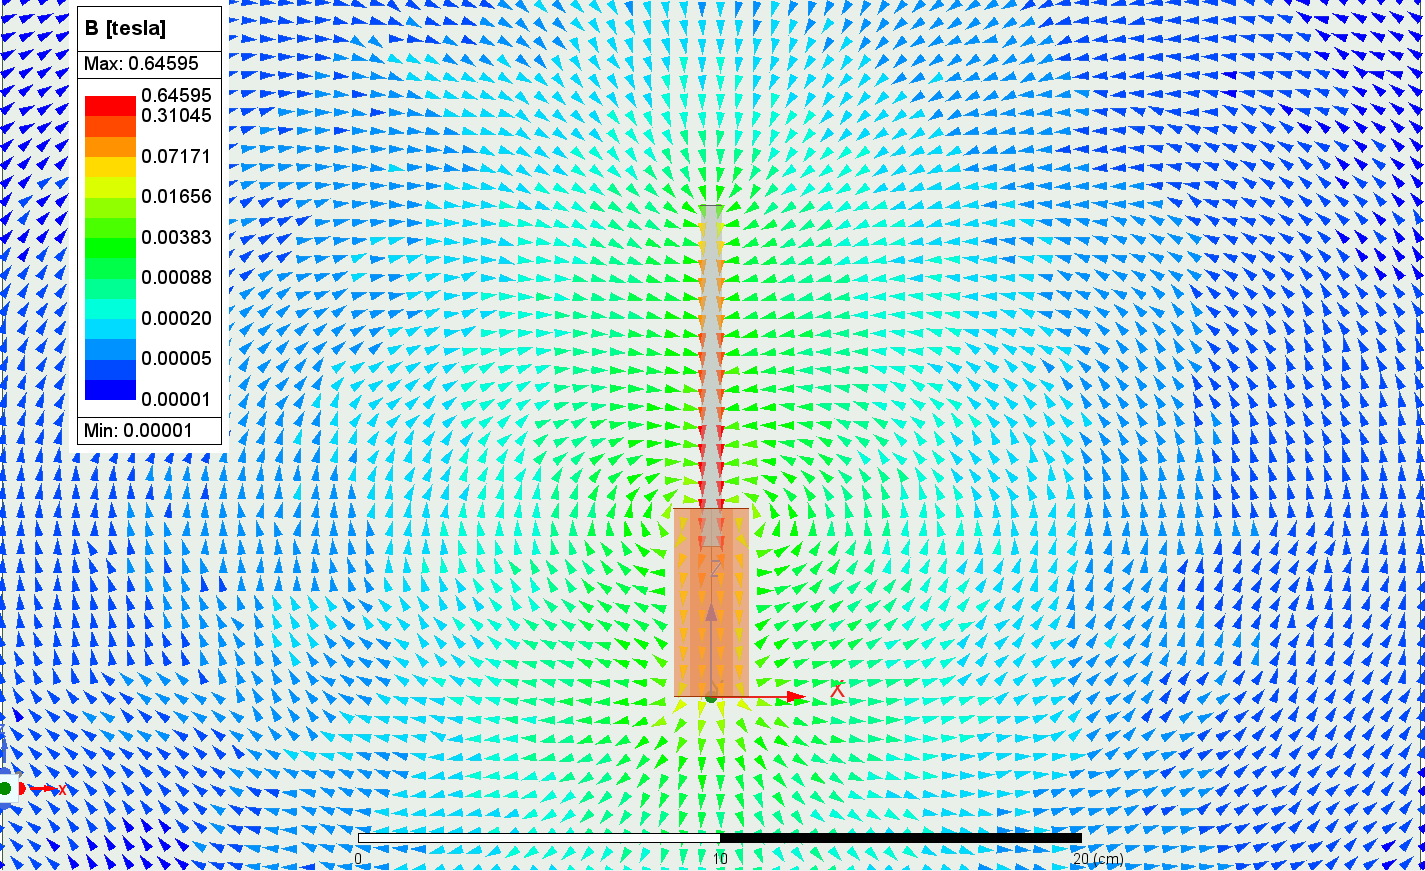
\includegraphics[width=14cm]{FigurasMemoria/fields8.PNG}
    \caption{Visualización de los campos magnéticos con la bobina energizada con \(I_{cc}=3.5~\text{A}\) y \(x=8/10 * h_c\).}
    \label{fig:fields8} %Para referenciar -> \ref{fig:figNum}
\end{figure}

Vemos que se puede apreciar perfectamente la forma descrita en las figuras \ref{fig:integralampere} y \ref{fig:electromagnet}, curvándose en los extremos del sistema pero permaneciendo bastante uniforme a lo largo de \(h_c\). Se muestra a continuación un detalle de los campos únicamente dentro de la bobina con la barra en la posición de la figura \ref{fig:fields8}:

\begin{figure}[H]
    \centering
    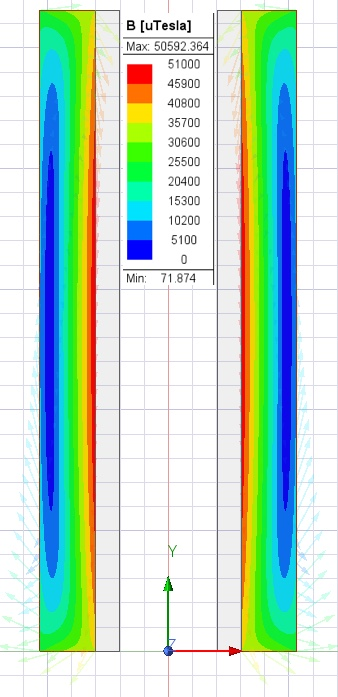
\includegraphics[width=3cm]{FigurasMemoria/fieldsDetail.jpg}
    \caption{Visualización de los campos magnéticos dentro del solenoide.}
    \label{fig:fieldsDetail} %Para referenciar -> \ref{fig:figNum}
\end{figure}

Además de visualizar los campos, ANSYS Maxwell\textsuperscript{\textregistered} permite añadir distintas medidas a la simulación, entre las que se encuentra la fuerza de atracción magnética. Realizando la simulación de nuevo para la configuración en 3D, se obtiene que la fuerza para la misma configuración de la gráfica de la figura \ref{fig:calcFsetupBase} es igual a:

\begin{table}[h]
    \centering
    \begin{tabular}{|c|c|c|c|c|}
        \hline
        & \(F_x\) & \(F_y\) & \(F_z\) & \(F_{tot}\) \\
        \hline
        \(F_{ANSYS}\) & 0,0012 & -0,0069 & -1,0553 & 1,0553 \\
        \hline
    \end{tabular}
    \caption{Fuerzas de atracción magnética en los diferentes ejes del espacio.}
    \label{tab:fuerzas}
\end{table}

\subsection{Simulaciones transitorias}
Una vez observados los campos de manera estacionaria, el siguiente paso es conseguir la variación de los valores de fuerza con la posición del vástago, además sin forzar este movimiento. Es decir, especificar la región de movimiento y los valores de alimentación de la bobina y dejar que ANSYS Maxwell\textsuperscript{\textregistered} genere el movimiento y nos de información acerca de la fuerza y velocidad experimentadas por el vástago. Al realizar esto con el modelo 3D, ANSYS Maxwell\textsuperscript{\textregistered} devolvía un error fatal probablemente debido a que los ordenadores en los que se estaba realiando la simulación no eran lo suficientemente potentes. Se recurrió entonces a la utilización exclusiva de la geometría en 2D, la que dio resultados tanto de movimiento como fuerza. Para llegar a los últimos resultados, se realizaron varias simulaciones con varias configuraciones temporales diferentes, las cuales se muestran a continuación:
\subsection*{Configuración 1}
La primera configuración transitoria utilizada es:
\[
T_{sim}=150~ms \quad T_{step}=5~ms \to 30~steps
\]
\[
I(t=0)=3.5~A \quad I(t\geq 50~ms)=0~A
\]
\[
V_{coil}=13.1~V \quad R_{coil}=3.65~\Omega
\]
\[
m_{bar}=0.019~kg \quad v_{bar~ini}=0~ms^{-1}
\]
Las gráficas resultantes de fuerza-corriente y velocidad-posición son:
\begin{figure}[H]
    \centering
    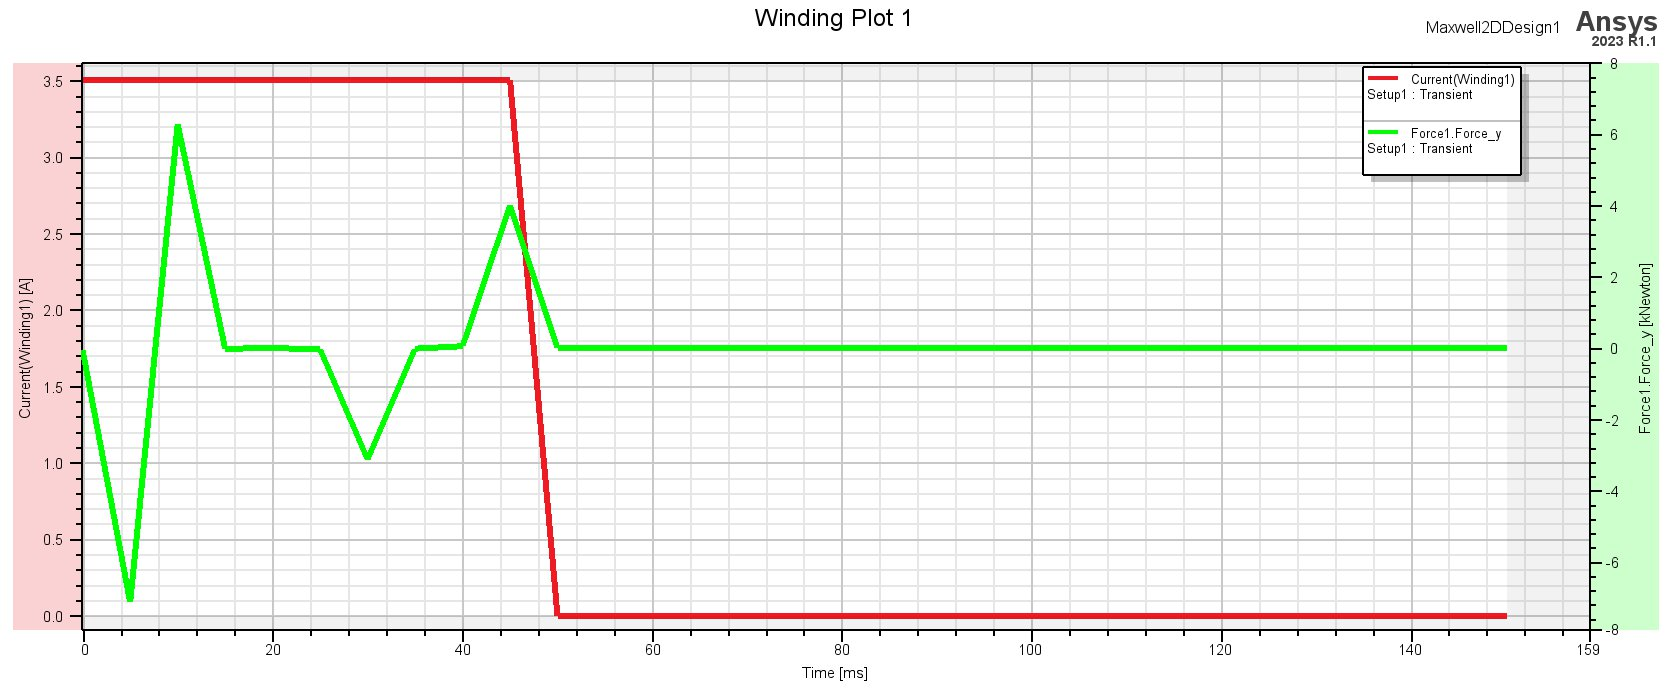
\includegraphics[width=13cm]{FigurasMemoria/S1CurrentForce.jpg}
    \caption{Fuerza (verde) y corriente (rojo) en función del tiempo de la configuración 1.}
    \label{fig:S1CurrentForce} %Para referenciar -> \ref{fig:figNum}
\end{figure}
\begin{figure}[H]
    \centering
    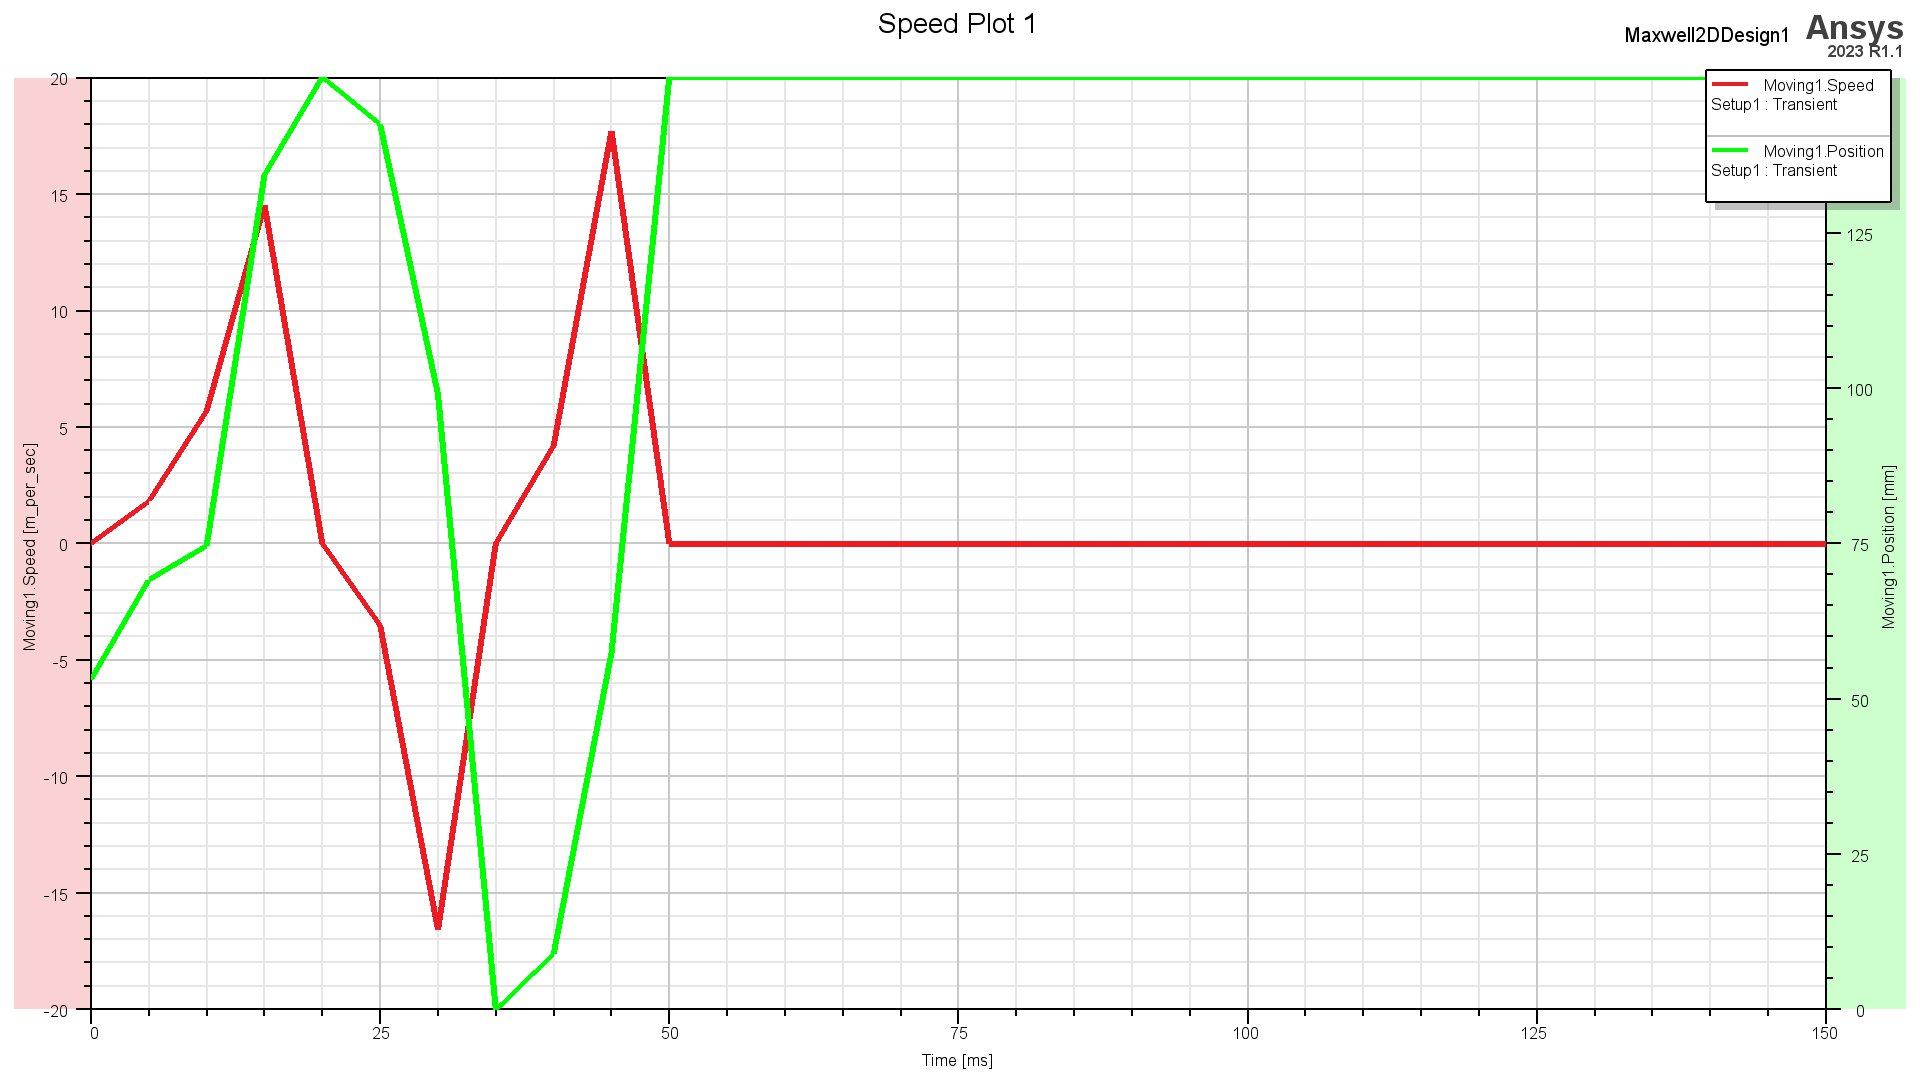
\includegraphics[width=10cm]{FigurasMemoria/S1SpeedPosition.jpg}
    \caption{Posición (verde) y velocidad (rojo) en función del tiempo de en la configuración 1.}
    \label{fig:S1SpeedPosition} %Para referenciar -> \ref{fig:figNum}
\end{figure}
Como se puede observar en las figuras \ref{fig:S1CurrentForce} y \ref{fig:S1SpeedPosition}, \(T_{sim}\) es muy largo ya que la mayor parte del tiempo no ocurre nada. También es destacable que existen oscilaciones, lo que indica que la bobina está siendo alimentada durante demasiado tiempo y está siendo retenida en el centro.


\subsection*{Configuración 2}
La segunda configuración transitoria utilizada es:
\[
T_{sim}=75~ms \quad T_{step}=0.6~ms \to 125~steps
\]
\[
I(t=0)=3.5~A \quad I(t\geq 30~ms)=0~A
\]
\[
V_{coil}=13.1~V \quad R_{coil}=3.65~\Omega
\]
\[
m_{bar}=0.019~kg \quad v_{bar~ini}=0~ms^{-1}
\]
Las gráficas resultantes de fuerza-corriente y velocidad-posición son:
\begin{figure}[H]
    \centering
    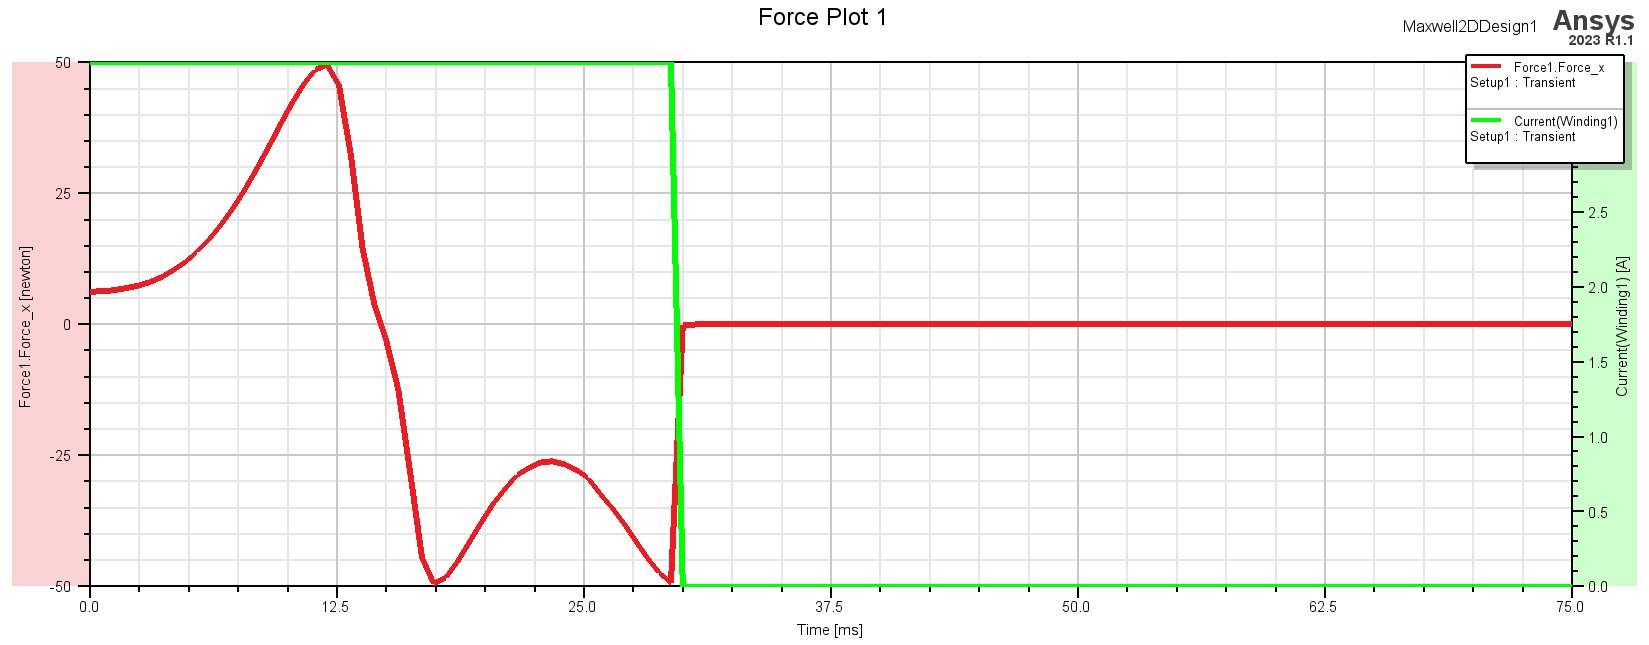
\includegraphics[width=13cm]{FigurasMemoria/S2ForceCurrent.jpg}
    \caption{Fuerza (rojo) y corriente (verde) en función del tiempo de la configuración 2.}
    \label{fig:S2ForceCurrent} %Para referenciar -> \ref{fig:figNum}
\end{figure}
\begin{figure}[H]
    \centering
    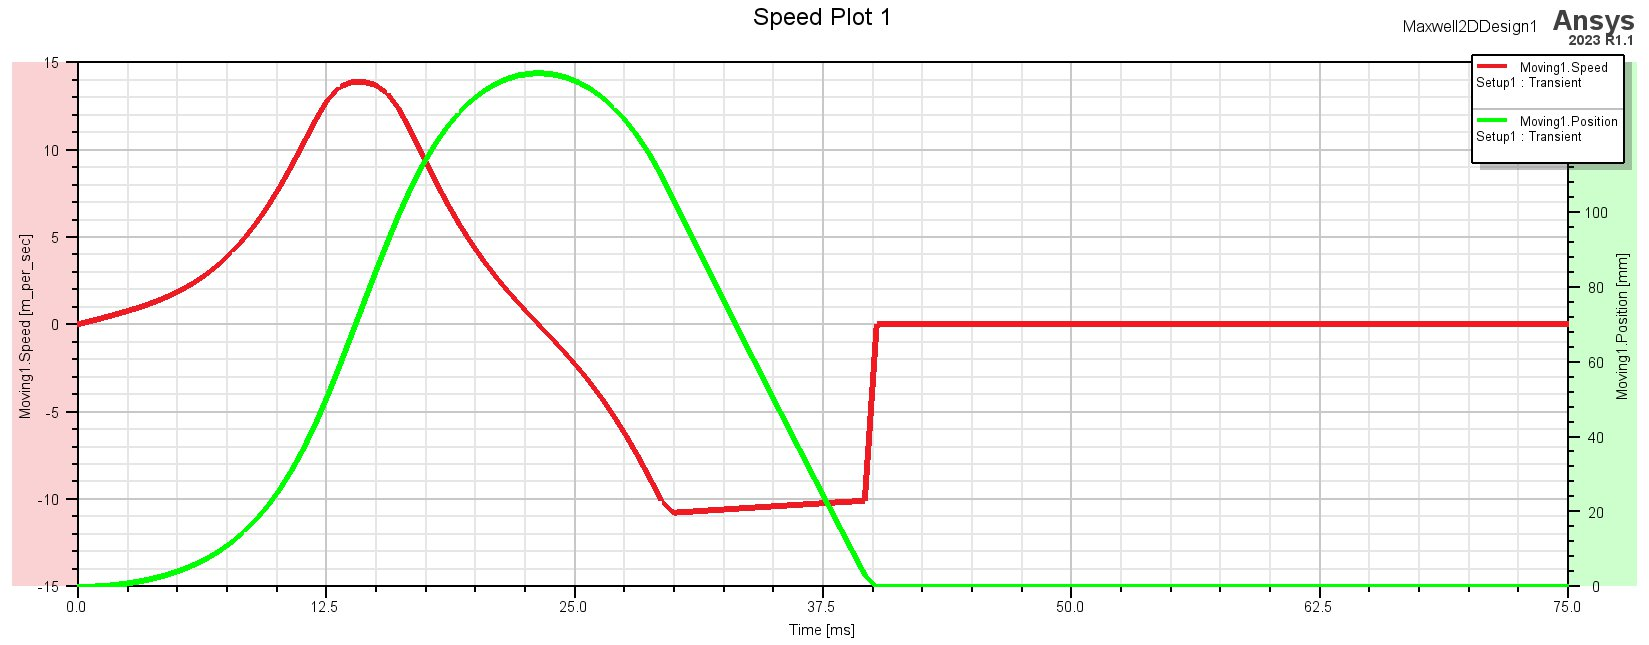
\includegraphics[width=13cm]{FigurasMemoria/S2SpeedPosition.jpg}
    \caption{Posición (verde) y velocidad (rojo) en función del tiempo de la configuración 2.}
    \label{fig:S2SpeedPosition} %Para referenciar -> \ref{fig:figNum}
\end{figure}
En la segunda configuración, se utilizó un timestep muy pequeño para poder observar con precisión el movimiento del vástago. Se observa más ajustado el tiempo de simulación, aunque el tiempo de alimentación de la bobina sigue siendo muy elevado ya que el vástago sigue oscilando, aunque ya solo lo hace una vez. 

\subsection*{Configuración 3}
La tercera configuración transitoria utilizada es:
\[
T_{sim}=25~ms \quad T_{step}=1~ms \to 25~steps
\]
\[
I(t=0)=3.5~A \quad I(t\geq 15~ms)=0~A
\]
\[
V_{coil}=13.1~V \quad R_{coil}=3.65~\Omega
\]
\[
m_{bar}=0.019~kg \quad v_{bar~ini}=0~ms^{-1}
\]
Las gráficas resultantes de fuerza-corriente y velocidad-posición son:
\begin{figure}[H]
    \centering
    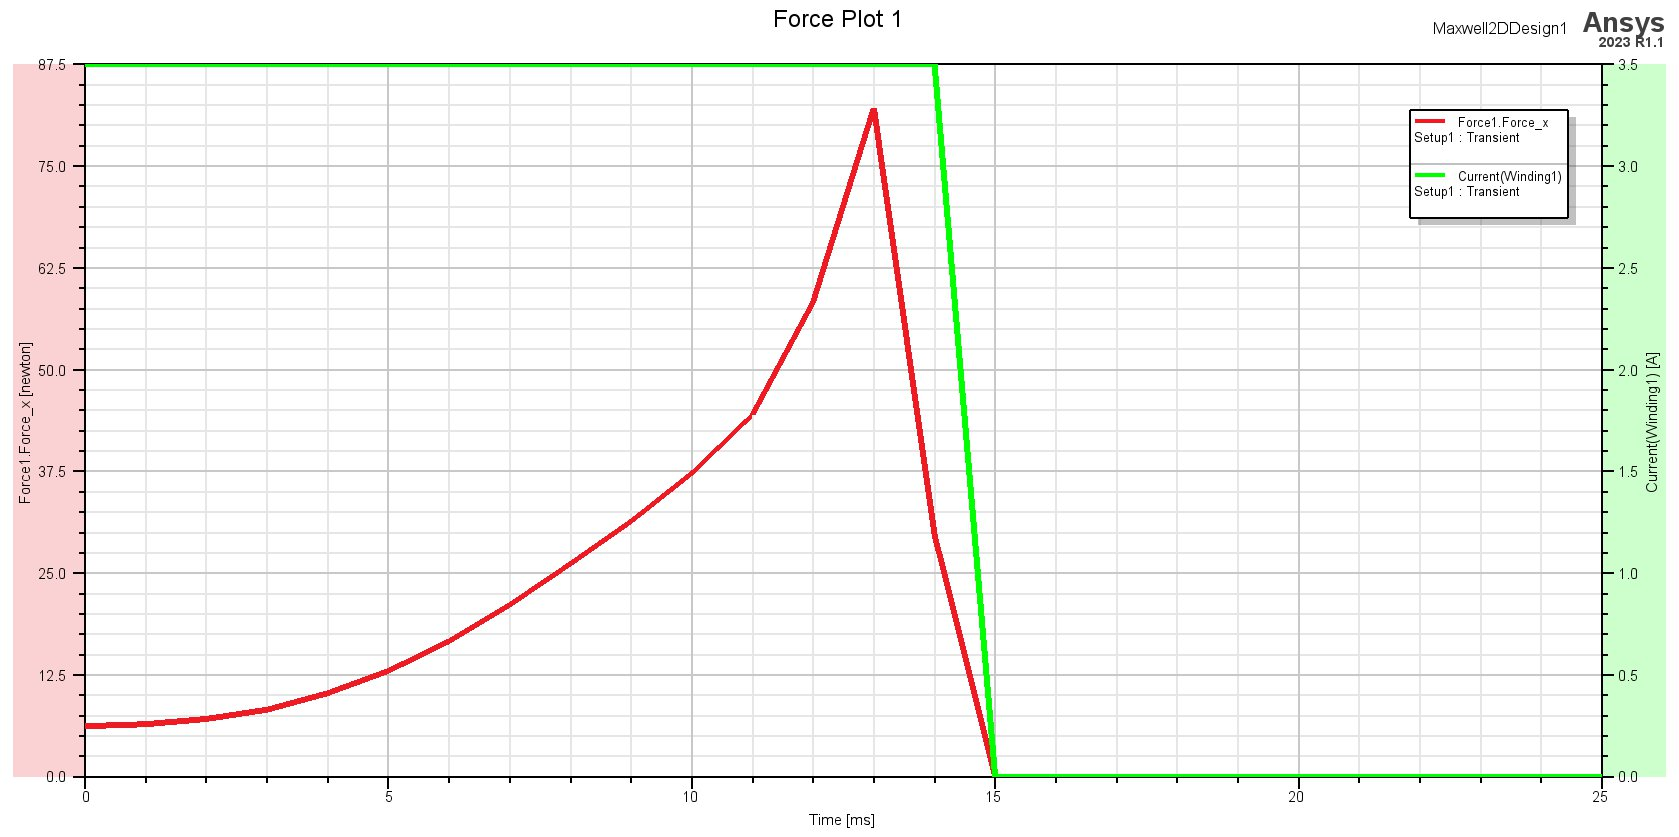
\includegraphics[width=13cm]{FigurasMemoria/S3ForceCurrent.jpg}
    \caption{Fuerza (rojo) y corriente (verde) en función del tiempo de la configuración 3.}
    \label{fig:S3ForceCurrent} %Para referenciar -> \ref{fig:figNum}
\end{figure}
\begin{figure}[H]
    \centering
    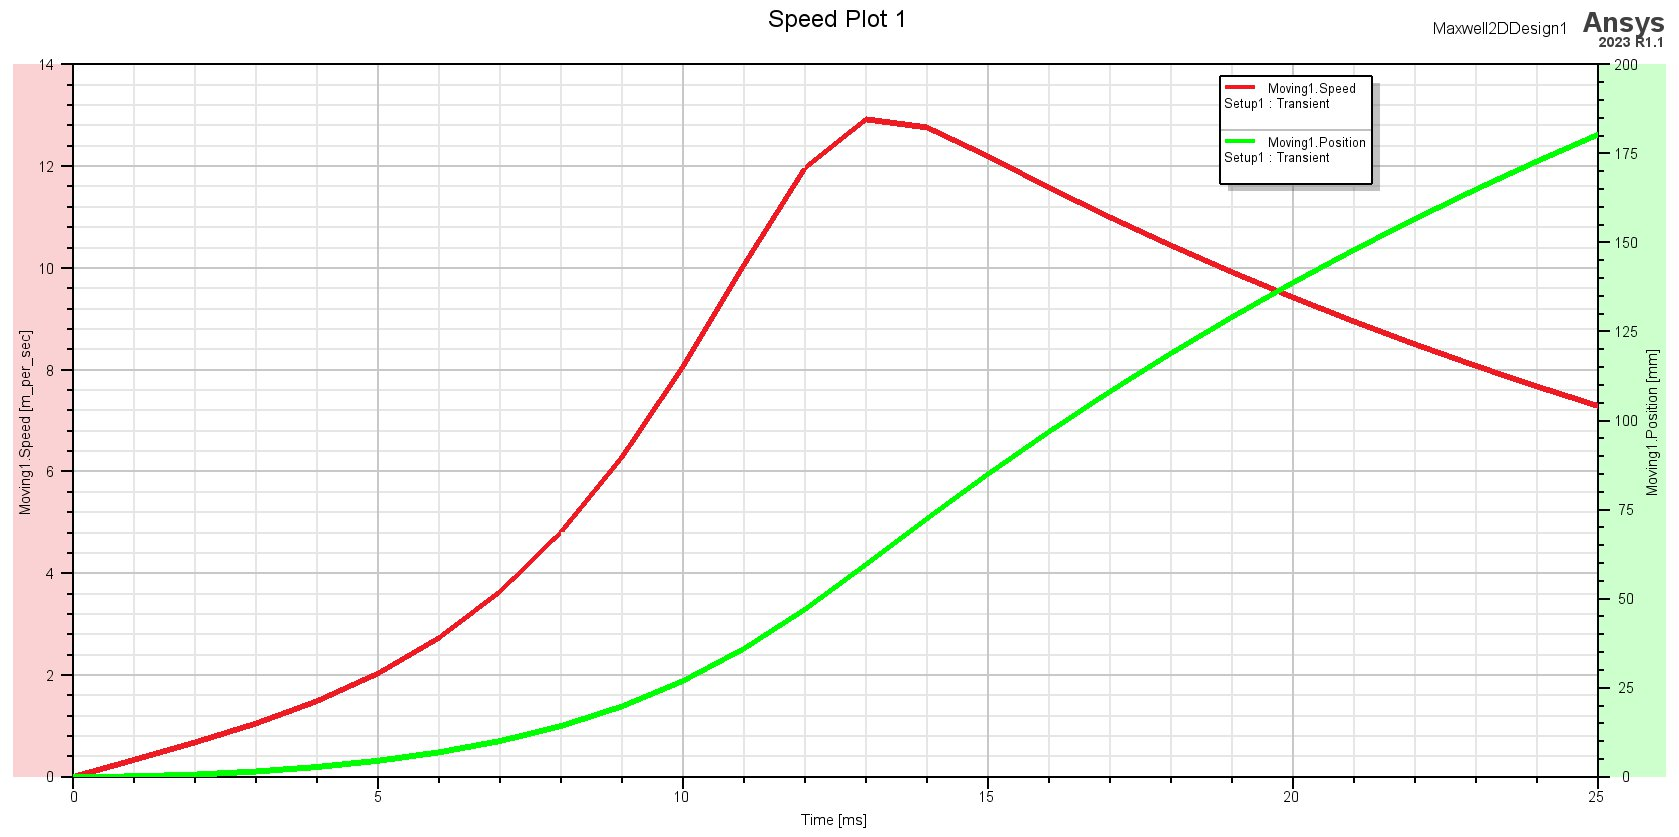
\includegraphics[width=13cm]{FigurasMemoria/S3SpeedPos.jpg}
    \caption{Posición (verde) y velocidad (rojo) en función del tiempo de la configuración 3.}
    \label{fig:S3SpeedPos} %Para referenciar -> \ref{fig:figNum}
\end{figure}

Esta configuración proporciona la evolución de la fuerza según el sistema que queremos crear, dejando de alimentar la bobina antes de que los centros estén alineados y permitiendo que el vástago siga avanzando por inercia, lo cual podemos comprobar observando la gráfica en la figura \ref{fig:S3SpeedPos}, en la que la posición no decrece en ningún momento. Sin embargo, los resultados de la magnitud de la fuerza no son verosímiles, pues son 40 veces mayores (\(F_{max}\approx 80~N\)) a la fuerza obtenida en la prueba de referencia (figura \ref{fig:dinamometro}).

Con esto se dará por finalizado el apartado de simulaciones. Aunque se ha encontrado una configuración que imita correctamente el comportamiento del sistema, los resultados obtenidos no son precisos en términos de magnitud. Dado que no se ha logrado avanzar en la mejora de la precisión de los resultados, se ha decidido no continuar dedicando más tiempo a afinar esta configuración. Se analizará en detalle lo obtenido en el apartado de validación de modelos (\ref{sec:resultados}).